\section{Introduction}
\label{section:intro}
Although enormous amounts of data exist in ``well-behaved'' formats such
as XML and relational databases, massive amounts also exist in
non-standard or \textit{ad hoc} data formats. \figref{figure:data-sources}
gives some sense of the range and pervasiveness of such data.
Ad hoc data comes in many forms: ASCII, binary, EBCDIC, and mixed
formats.  It can be fixed-width, fixed-column, variable-width, or even
tree-structured. It is often quite large, including some data sources
that generate over a gigabit per second~\cite{gigascope}. It frequently
comes with incomplete and/or out-of-date documentation, and there are
almost always errors in the data.  Sometimes these errors are the most
interesting aspect of the data, \eg{}, in log files where
errors indicate that something is going wrong in the associated
system.

\begin{figure}
\begin{center}
\begin{tabular}{l|l}
\hline
\textbf{Name} : Use   &  Representation               \\ \hline
\textbf{Web server logs (CLF)}:  &  Fixed-column ASCII records \\ 
Measure web workloads &                             \\ \hline
\textbf{AT\&T provisioning data}: & Variable-width ASCII records  \\ 
Monitor service activation &                              \\ \hline
\textbf{Call detail}: Fraud detection  &  Fixed-width binary records \\  \hline 
\textbf{AT\&T billing data}: & Various Cobol data formats  \\ 
Monitor billing process   &                             \\ \hline
%IP backbone data:  & ASCII   \\
%Monitor network performance  &        \\ \hline
\textbf{Netflow}:                        & Data-dependent number of     \\ 
Monitor network performance  & fixed-width binary records  \\ \hline
\textbf{Newick}:   Immune                 & Fixed-width ASCII records \\ 
system response simulation & in tree-shaped hierarchy\\ \hline                                
\textbf{Gene Ontology}:             & Variable-width ASCII records \\
Gene-gene correlations     & in DAG-shaped hierarchy \\ \hline
%HL7:             & Variable-width ASCII records \\
%Medical lab results     &  \\ \hline
\textbf{CPT codes}: Medical diagnoses & Floating point numbers \\ \hline
\textbf{SnowMed}: Medical clinic notes & Keyword tags  \\ 
\end{tabular}

\caption{Selected ad hoc data sources.}
\label{figure:data-sources}
\end{center}
\end{figure}



The lack of standard tools for processing ad hoc data forces
analysts to roll their own tools, leading to scenarios such as the
following.  An analyst receives a new ad hoc data source containing
potentially interesting information and a list of pressing questions
about that data.  Could she please provide the answers to the
questions as quickly as possible, preferably last week?  The
accompanying documentation is outdated and missing important
information, so she first has to experiment with the data to discover
its structure.   Eventually, she understands the data well enough to hand-code a
parser, usually in \C{} or \perl{}.  Pressed for time, she interleaves
code to compute the answers to the supplied questions with the parser.
As soon as the answers are computed, she gets a new data source and a
new set of questions to answer.

Through her heroic efforts, the data analyst answered
the necessary questions, but the approach is deficient in many
respects.  
The analyst's hard-won understanding of the data ended up embedded in
a hand-written parser, where it is difficult for others to benefit
from her understanding.
The parser is likely to be brittle with respect to changes in the
input sources.  Consider, for example, how tricky it is to
figure out which \$3's should be \$4's in a \perl{} parser when a new
column appears in the data.
Errors in the data also pose a significant challenge in hand-coded
parsers.  If the data analyst thoroughly checks for errors, then
the error checking code dominates the parser, making it even more
difficult to understand the semantics of the data format.  If she is not thorough,
then erroneous data can escape undetected, potentially (silently!)
corrupting down-stream processing.
Finally, during the initial data exploration and in answering the
specified questions, the analyst had to code \textit{how to compute}
the questions rather than being able to express the queries in a
declarative fashion. 
Of course, many of these pitfalls can be avoided with careful design
and sufficient time, but such luxuries are not available to the analyst.
However, with the appropriate tool support, many aspects of this
process can be greatly simplified.


\cut{
Story: Start with data analyst perspective.  Has ad hoc data source
and a set of questions that he'd like to ask about it.  But the
structure of the data source can change over time and he does not want
his questions to be brittle.  E.g., if using Perl, you don't want to
have to change the Perl program each time a small change occurs in the
structure of the data.  Data sources can be large.  Format conversion
from ad hoc to standard format.  

We had/have solutions to each of these problems in isolation: \pads{} and
\Galax{}.  Story of this paper is the interaction of these systems to
solve all the data analyst's problems simultaneously. 
1. Need to describe it (PADS)
2. Query it and convert to XML (XQuery) 
3. Deal with scale.
Problem focused, not tool focused. 

}

We have two tools, \pads{}~\cite{padsmanual,pldi05} and
\Galax{}~\cite{galaxmanual,galax}, each of which addresses aspects of
the analyst's problem in isolation.  The \pads{} system allows
analysts to describe ad hoc data sources declaratively and then
generates error-aware parsers and tools for manipulating the sources,
including statistical profiling tools.  Such support allows the
analyst to produce a robust, error-aware parser quickly.  The \Galax{}
system supports declarative querying of XML
via XQuery.  If Galax could be applied to ad hoc data, it 
would allow the analyst first to explore the data and then to produce
answers to her questions.  It would also support converting the data
into XML to facilitate downstream processing with XML-based tools if
she so desired.

In this work, we strove to integrate \pads{} and \Galax{}
to solve the analyst's data-management problems for the large ad hoc
data sources that we have seen in practice.
We describe our experience designing and implementing
\padx{}\footnote{%
  Pronounced ``paddocks'', an enclosed area for exercising race
  horses.},
a synthesis and extension of \pads{} and 
\Galax{}.  Figure~\ref{figure:padx-arch1} depicts \padx{} from the
analyst's perspective.  The analyst provides a \pads{} description of
her ad hoc source, which is compiled into a library of components for
parsing her data and for viewing and querying it as XML.  The
resulting libraries are linked together with the \pads{} and \Galax{}
runtime systems into one \padx{} query executable, called a ``query
corral.\footnote{%
   The equestrian metaphor is intentional: Getting these systems to
   work together is like corralling race horses!}''
At query time, the analyst provides her ad hoc data sources and her query
written in XQuery, and \padx{} produces the query's results.
\begin{figure}
\begin{center}
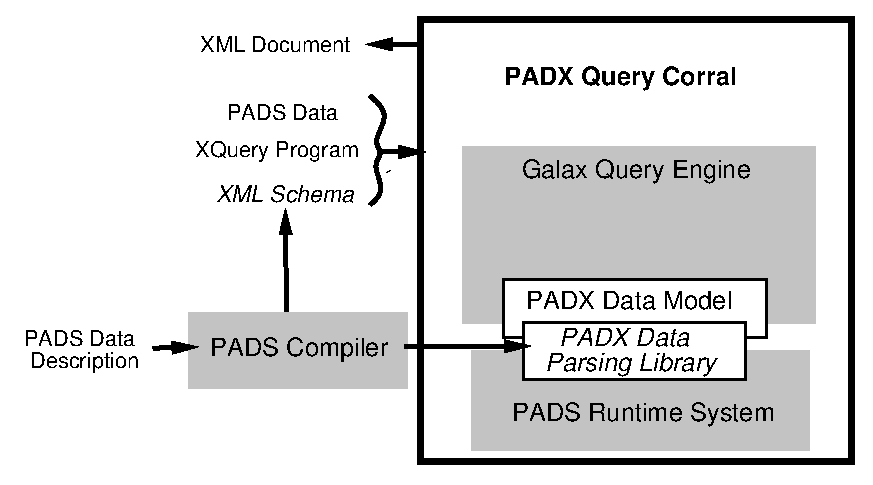
\epsfig{file=padx-arch1.ps,width=0.25\textwidth}
\end{center}
\caption{Data analyst's view of \padx{}}
\label{figure:padx-arch1}
\end{figure}

Building \padx{} presented several problems. The first was semantic:
We had to decide how to view ad hoc data as XML and how to express
this view as a mapping from the \pads{} type system to XML Schema, the
basis of XQuery's type system.  A second problem involved systems
design and engineering.  Building \padx{} required evolving \pads{}
and \Galax{} in parallel, modifying the implementation of \Galax{} to
support an abstract data model so that \Galax{} could view non-XML
sources as XML, and augmenting \pads{} with the ability to generate
concrete instances of this data model.  Our solutions to these
problems, which were necessary to build a working system, are
described in Sections~\ref{section:galax} and~\ref{section:padx}.  A
third problem involves the scale of data and efficiency of queries, in
particular, how to efficiently evaluate complex queries over large
sources.  Section~\ref{section:performance} describes how \padx{}
currently handles large sources and the problems that we face
with respect to data scale and query performance.

We begin with a more detailed account of a scenario that illustrates
the data management tasks faced by AT\&T data analysts and how \padx{}
simplifies these 
tasks.  We then crack open the \padx{} architecture, first describing
\pads{} and \Galax{} in isolation, and then describing our solutions
to the problems described above.  
We conclude with related work and a discussion of open problems.

\cut{
In Section~\ref{section:padx}, we describe the embedding of the \pads{}
type system in XML Schema and the XML view of ad hoc data available in
XQuery.

\scream{Do we want to explain that \padx{} is an example of a
(semi)-compiled query architecture and what that means?  Say something
about soundness of schema, data, and queries.  And point out that some
of these problems were solved in the implementations of object-oriented
databases (25 years ago!)}

Architecture of \padx{}.  Supports both non-materialized and virtual  
querying of \pads{} data.  Example: dot query.  User gets to choose
whether to query materialized or virtual XML data.  Appropriate model
depends on query work load and other processes in work flow.  We
support both (!)

Potential benefits: leverage speed of
XQuery processor over native XML document.  Potential costs: same as
having using a materialized view of a database.  ``Staleness'' of XML,
multiple copies, extra time to convert to XML.  Work-load/cost-based
optimization problem.  Tradeoffs between materializing XML document
and querying it multiple times.  Our architecture appropriate for
certain problems.  Data gets regenerated every week or so.  Already
Gigabytes of data.  Could use \pads{} and \Galax{} separately to same
effect.
}
 
\cut{
Systems were developed in parallel.  Solving the above problem
required some additional engineering: implementation of \Galax{}'s
abstract data model on top of \pads{} parsing-read functions.  
Hence, we are going to talk about both systems followed by their
synthesis. 

Don't want to explain each system as isolated entities, but show their
interaction---symbiotic relationship that enhances the functionality
of each system.  Explain an interaction between the systems.

Data management standpoint: Vast amounts of data sources that are not
in XML.  Even if you want to view/materialize them in XML, you still
have to get a handle on the data.  Thus, the necessity for \pads{}. 

Programming language spin: a declarative data description, run
compiler, and get parser and related tools. 

XML standpoint: 
XQuery intended to 
\pads{} is an ideal target for \Galax{} as we get a statically typed view of the
non-XML data, and therefore we can statically type check any queries
over the \pads{} data.

There are a couple of stories here.  One is a semantic story: XQuery
is a reasonable query language for \pads{}.  Both represent
semi-structured data.  Error-aware computing by revealing PD in 
XML virtual view.  Question: XML Schema can describe \pads{} types, 
but what about vice versa? Embedding of \pads{} types in XML Schema. 


The other story is about laziness : in \Galax{}'s
algebraic query plans, in its tree data model, and in \padx{}'s
implementation of \Galax{}'s tree data model.  Laziness supports
scalability of data (and queries?).  Last (small) story is about
\padx{}'s compiled data model---(almost) constant time access to named
fields.

How to support semantic story?  Show mapping from \pads{} types to XML
Schema.  Show realization of pd info.  Show semantics/expressiveness
of queries. 

How to support the importance of laziness? (Or is this too obvious?)
Show scalability of smart loading over bulk loading.  Show improvement
of compiled name access over interpreted name access. 
}

\subsection{Data-management scenario}
\label{subsec:example}

%\figref{figure:dibbler-records}
In the telecommunications industry, the term \textit{provisioning} refers to
the process of converting an order for phone service into the
actual service.  This process is complex, involving many interactions
with other companies.  To discover potential problems proactively, the \dibbler{}
project tracks AT\&T's provisioning process by compiling weekly
summaries of the state of certain types of phone service orders.
These summaries, which are stored in flat ASCII text files, can
contain more than 2.2GB of data per week.

The summaries store the processing date
and one record per order.  Each order record contains a header
followed by a nested sequence of events.  The header has 13 pipe
separated fields: the order number, AT\&T's internal order number, the
order version, four different telephone numbers associated with the
order, the zip code, a billing identifier, the order
type, a measure of the complexity of the order, an unused field, and
the source of the order data.  Many of these fields are optional, in
which case nothing appears between the pipe characters.  The billing
identifier may not be available at the time of processing, in which
case the system generates a unique identifier, and prefixes this value
with the string ``no\_ii'' to indicate the number was generated. The
event sequence represents the various states a service order goes
through; it is represented as a new-line terminated, pipe separated
list of state, timestamp pairs.  There are over 400 distinct states
that an order may go through during provisioning.  It may be apparent from
this description that English is a poor language for describing data
formats!

\begin{figure*}
\begin{small}
\begin{center}
\begin{verbatim}
0|15/Oct/2004:18:46:51
9152|9152|1|9735551212|0||9085551212|07988|no_ii152272|EDTF_6|0|APRL1|DUO|10|16/Oct/2004:10:02:10
9153|9153|1|0|0|0|0||152268|LOC_6|0|FRDW1|DUO|LOC_CRTE|1001476800|LOC_OS_10|17/Oct/2004:08:14:21
\end{verbatim}
\caption{Tiny example of \dibbler{} provisioning data.}
\label{figure:dibbler-records}
\end{center}
\end{small}
\end{figure*}

The analyst's first task is to write a parser for the
\dibbler{} data  format.  Like many ad hoc data sources, \dibbler{} data
can contain unexpected or corrupted values, so the
parser must handle errors robustly to avoid corrupting the results of
analyses.  \cut{Today, parsers for ad hoc formats are often hand-crafted in 
\perl{} or \C{}.  Unfortunately, writing parsers this way is tedious and
error prone, complicated by the lack of documentation, convoluted
encodings designed to save space, and the need to produce efficient
code.  Moreover, the analyst's hard-won understanding of the data ends
up embedded in parsing code, making long-term maintenance difficult
for the original writers and sharing the knowledge with others nearly
impossible.}
With \pads{}, the analyst writes a declarative data description of the
physical layout of her data.  The language also permits the analyst to
describe expected semantic properties of her data so that deviations
can be flagged as errors. The intent is to allow an analyst to capture
in a \pads{} description all that she knows about a given data source.

\figref{figure:dibbler} gives the \pads{} description for the
\dibbler{} data format.  In \pads{} descriptions, types are declared
before they are used, so the type that describes the entire data
source, \cd{summary\_t}, appears at the bottom of the description (Line~42).  In
the next section, we use this example to give an overview of
the \pads{} language.  Here, we simply note that the data analyst
writes this description, and the \pads{} compiler produces
customizable \C{} libraries and tools for parsing, manipulating, and
summarizing the data.  The fact that useful software artifacts are
generated from \pads{} descriptions provides strong incentive for
keeping the descriptions current, allowing them to serve as living
documentation.

\begin{figure}
\begin{small}
\begin{code}
{ 1}. \kw{Precord} \kw{Pstruct} summary\_header\_t \{
{ 2}.  "0|";
{ 3}.  Punixtime tstamp;
{ 4}. \};
\mbox{}
{ 5}. \kw{Pstruct} no\_ramp\_t \{
{ 6}.  "no\_ii";
{ 7}.  Puint64 id;
{ 8}. \};
\mbox{}
{ 9}. \kw{Punion} dib\_ramp\_t \{
{10}.   Pint64     ramp;
{11}.   no\_ramp\_t  genRamp;
{12}. \};
\mbox{}
{13}. \kw{Pstruct} order\_header\_t \{
{14}.        Puint32             order\_num;
{15}.  '|';  Puint32             att\_order\_num;
{16}.  '|';  Puint32             ord\_version;
{17}.  '|';  \kw{Popt} pn\_t           service\_tn;
{18}.  '|';  \kw{Popt} pn\_t           billing\_tn;
{19}.  '|';  \kw{Popt} pn\_t           nlp\_service\_tn;
{20}.  '|';  \kw{Popt} pn\_t           nlp\_billing\_tn;
{21}.  '|';  \kw{Popt} Pzip           zip\_code;
{22}.  '|';  dib\_ramp\_t          ramp;
{23}.  '|';  Pstring(:'|':)      order\_type;
{24}.  '|';  Puint32             order\_details;
{25}.  '|';  Pstring(:'|':)      unused;
{26}.  '|';  Pstring(:'|':)      stream;
{27}. \};
\mbox{}
{28}. \kw{Pstruct} event\_t \{
{29}.        Pstring(:'|':)    state;   
{30}.   '|'; Punixtime         tstamp;
{31}. \};
\mbox{}
{32}. \kw{Parray} event\_seq\_t \{
{33}.   event\_t[] : \kw{Psep}('|') && \kw{Pterm}(\kw{Peor});
{34}. \};
\mbox{}
{35}. \kw{Precord} \kw{Pstruct} order\_t \{
{36}.        order\_header\_t  order\_header;
{37}.   '|'; event\_seq\_t     events;
{38}. \};
\mbox{}
{39}. \kw{Parray} orders\_t \{
{40}.   order\_t[];
{41}. \};
\mbox{}
{42}. \kw{Psource} \kw{Pstruct} summary\_t\{
{43}.   summary\_header\_t  summary\_header;
{44}.   orders\_t          orders;
{45}. \};
\end{code}
\end{small}
\caption{\pads{} description for \dibbler{} provisioning data.}
\label{figure:dibbler}
\end{figure}

Analysts working with ad hoc data often want to query their data.  
Questions posed by the \dibbler{} analyst include ``Select all
orders starting within a certain time window,'' ``Count the number of
orders going through a particular state,'' and ``What is the average
time required to go from a particular event state to another
particular event state''.  Such queries are useful for rapid
information discovery and for vetting errors and anomalies in data
before that data proceeds to a down-stream process or is loaded into a 
database.

\begin{figure}
\begin{small}
\begin{code}
\kw{(: Return orders started in October 2004 :)}
$pads/Psource/orders/elt[events/elt[1]
  [tstamp/rep {>=} {xs:dateTime}("2004-10-01:00:00:00")
{and} tstamp/rep {<} {xs:dateTime}("2004-11-01:00:00:00")]]
\end{code}
\end{small}
\caption{Query applied to \dibbler{} provisioning data.}
\label{figure:dibbler-query}
\end{figure}

With \padx{}, the analyst
writes declarative XQuery expressions to query her ad hoc data source.
Because XQuery is designed to manipulate semi-structured data, its
expressiveness matches ad hoc data sources well.  
As a Turing-complete language, XQuery is powerful
enough to express all the questions above.  For example,
Figure~\ref{figure:dibbler-query} contains an XQuery expression that
produces all orders that started in October, 2004.  In
Section~\ref{section:padx}, we discuss in more detail why XQuery is an appropriate
query language for ad hoc data.  One benefit is that XQuery queries may be
statically typed, which helps detect common errors at compile time.
For example, static typing would raise an error if the path expression
in Figure~\ref{figure:dibbler-query} referred to \cd{ordesr} instead
of \cd{orders}, or if the analyst erroneously compared the timestamp
value in \cd{tstamp} to a string.
